\documentclass[11pt,a4paper]{article}
\usepackage[utf8]{inputenc}
\usepackage[T1]{fontenc}
\usepackage[english]{babel}
\usepackage{lmodern,microtype,amsmath,amssymb,booktabs,array,graphicx,xcolor,geometry,setspace,float,longtable}
\usepackage{tikz}
\usetikzlibrary{arrows.meta,positioning}
\usepackage[font=small,labelfont=bf]{caption}
\usepackage[hidelinks]{hyperref}
\geometry{margin=25mm}
\setstretch{1.16}
\setlength{\parskip}{0.35em}
\setlength{\parindent}{1.2em}
\setlength{\emergencystretch}{2em}
\makeatletter
\setlength{\@fptop}{0pt}
\setlength{\@fpsep}{18pt}
\setlength{\@fpbot}{0pt plus 1fil}
\makeatother
\definecolor{reused}{HTML}{1755A0}
\definecolor{revised}{HTML}{B85A00}
\definecolor{added}{HTML}{B02228}
\newcommand{\old}[1]{{\color{reused}#1}}
\newcommand{\rev}[1]{{\color{revised}#1}}
\newcommand{\new}[1]{{\color{added}#1}}
\newenvironment{addition}{\begingroup\color{added}}{\endgroup}
\newcommand{\pp}{percentage points}
\newcommand{\figroot}{../../3. Output/two_papers_2026-09-21/figures/}
\newcommand{\draftlegend}{\begin{center}\small\color{black}Coauthor working draft --- 21 September 2026\\\old{Blue: wording retained verbatim.}\quad\rev{Orange: revised existing material.}\\\new{Red: new text or analysis.} Figure frames and captions indicate provenance; plotted colors do not.\end{center}}
\newcommand{\authors}{\old{Ignacio Garijo-Campos} \and \old{Antonio Alfonso} \and \old{Pablo Bra\~nas-Garza} \and \old{Diego Jorrat} \and \old{Angel Sanchez}}
\newcommand{\plot}[4]{\begin{figure}[!htbp]\centering\begingroup\color{#1}\setlength{\fboxsep}{2pt}\fbox{\includegraphics[width=.94\linewidth]{\figroot#2.png}}\caption{\textcolor{#1}{#3}}\label{#4}\endgroup\end{figure}}
\newcommand{\tabnote}[1]{\par\smallskip{\footnotesize\noindent\textit{Notes:} #1\par}}
\newcommand{\inputtab}[4]{\begin{table}[!htbp]\centering\begingroup\color{#1}\caption{\textcolor{#1}{#3}}\label{#4}\small\input{tables/#2.tex}\endgroup\end{table}}
\date{}

\title{\rev{The Decision to Hold Back: Student Information, Teacher Disagreement, and the Limits of Predictability}}
\author{\authors}
\begin{document}
\maketitle\draftlegend
\color{revised}
\begin{abstract}\color{added}
Why do teachers recommend grade repetition, and how much can their observable characteristics tell us about disagreement? A survey experiment with 2,705 teachers in Castilla-La Mancha, Spain, provides 22,124 recorded recommendations for standardized student profiles. The analysis separates the information associated with recommendations, disagreement about comparable profiles, and prediction of teachers' relative recommendation propensity. Within-teacher estimates are largest for failing three or more subjects (54.6 percentage points) and low basic competences (27.1 points). Two teachers evaluating the same recorded profile disagree in approximately 25.9 percent of response pairs. Nevertheless, observed professional characteristics and reported beliefs have limited predictive value. On a common sample of 2,156 teachers, repeated validation that constructs profile benchmarks exclusively from training teachers yields an out-of-fold $R^2$ of 3.0 percent for the full linear model and 0.6 percent for a random forest. Differences associated with educational stage, age, effort attribution, and resource skepticism therefore coexist with substantial unpredictability. Descriptive score terciles characterize the observed responses without identifying stable teacher types. The findings show the value of standardized cases for separating student composition from judgment, while limiting claims about the ability to identify more repetition-prone teachers from their observed backgrounds.
\end{abstract}
\noindent\textbf{Keywords:} grade repetition; teacher judgment; standardized vignettes; disagreement; prediction; educational inequality.

\section{Introduction}
The decision that a student should repeat a grade connects evidence about learning to a consequential educational recommendation. Identifying which evidence teachers use is one part of understanding this decision. Establishing whether teachers agree when they receive comparable information is another. A third question is whether a teacher's observable background and reported beliefs allow the researcher to anticipate the recommendation. These questions need not have the same answer: strong common responses to academic difficulties can coexist with disagreement that is difficult to predict.

Research on the consequences of grade repetition does not resolve how teachers arrive at recommendations. Estimated consequences vary across research designs, contexts, and comparison groups \cite{allen,goos}. Nor does disagreement necessarily mean that one teacher has misread the evidence. Teachers may differ in the benefits they expect from repetition, the alternatives they consider feasible, or the threshold of difficulty they regard as sufficient. Studying those judgments requires a design that separates the information presented from the students normally encountered by each teacher.

Administrative data make that separation difficult. Teachers and students are not usually matched at random, and the information available to a teacher extends beyond recorded test scores and background characteristics. A teacher who recommends repetition more frequently may simply teach students with different needs. Some teachers may rarely encounter particular social or academic circumstances. Standardized cases broaden the range of situations evaluated and make the presented information observable to the researcher. They improve comparability without reproducing every feature of an actual evaluation meeting.

We study recommendations from teachers in Castilla-La Mancha using profiles that vary in six recorded characteristics: gender, complex background, failed subjects, basic competences, absenteeism, and disciplinary problems. The retained analysis includes 2,705 teachers and 22,124 responses. We first estimate within-teacher differences associated with the profile characteristics. We then measure disagreement among respondents evaluating the same recorded card and construct a relative propensity to recommend repetition. Finally, we compare explanatory regressions with predictions for teachers held out from model estimation.

The findings reveal a pronounced hierarchy of student information. Three or more failed subjects increase the fitted recommendation probability by 54.6 percentage points; low mathematical or linguistic competences increase it by 27.1 points. Behavioral signals have smaller coefficients. At the same time, approximately one quarter of response pairs for an identical card disagree. Observable teacher characteristics account for only a small portion of variation in relative recommendation propensity. On a common sample, the most extensive linear specification explains 4.2 percent in sample and 3.0 percent out of sample. A flexible random forest yields an out-of-fold $R^2$ of 0.6 percent.

\new{The contribution is the combination of these three findings under common information. Existing research already documents the importance of academic performance. The more informative result is that substantial disagreement remains difficult to anticipate using the characteristics typically available to researchers and administrators, even when the students presented are standardized. This is a statement about the observed recommendation measure and available predictors; it does not establish that teachers are interchangeable, that judgment is arbitrary, or that stable differences are absent.}

\section{Related literature}
The first relevant literature concerns the consequences of retaining a student. Allen et al.\ \cite{allen} find that stronger research designs yield less negative retention effects than weaker designs, correcting a common reversal of their result. Goos et al.\ \cite{goos} document substantial heterogeneity across settings and methods in a broad review. These findings motivate studying how teachers evaluate repetition, but they do not supply a single correct answer to every vignette. The present outcome is a recommendation, not the causal effect of retention on later achievement.

A second literature investigates teachers' beliefs and judgments. Tomchin and Impara \cite{tomchin} examine the reasoning teachers use to justify retention. Bonvin \cite{bonvin} relates teacher attitudes and judgments to actual retention decisions. These studies establish that teachers' interpretations deserve attention alongside student performance. More recently, Klapproth and Beyte \cite{klapproth} use experimental vignettes to study grade-point averages, gender, failed subjects, and teacher attitudes. Their work is a close antecedent: experimental analysis of retention recommendations is not itself new. Our extension is to connect variation in multiple presented attributes with directly measured disagreement and a separate test of out-of-sample predictability in a larger teacher sample.

The distinction between beliefs, knowledge, and reported attitudes also matters \cite{pajares}. An association between a belief item and a recommendation does not show that changing the belief would change the decision. Here, several belief measures follow the decision task. We therefore use them to characterize and predict responses rather than as randomized explanations of behavior.

\new{Methodologically, the study draws on the logic of multidimensional vignette experiments \cite{conjoint}. Interpretation depends on the profiles actually represented and the distribution over which a comparison is averaged. Standardizing information strengthens internal comparisons, but external validity requires separate evidence. Validation of vignette choices against real behavior in other domains \cite{validation} does not validate retention recommendations automatically. Finally, the distinction between fitting associations and predicting new observations motivates our validation procedure \cite{prediction}. Random forests \cite{rf} provide a flexible comparison, and SHAP summaries \cite{shap} describe the fitted prediction function rather than the causal importance of teacher characteristics.}

\section{Study design and measurement}
\subsection{Participants and recommendation task}
The study concerns primary and secondary teachers in Castilla-La Mancha, Spain. The initial study plan specifies recruitment through the regional education authority and schools forwarding an online survey to teachers. Participation is voluntary, so a broad invitation frame does not imply a probability sample of responding teachers. The raw export contains 4,942 records; the retained cleaned file contains 4,553, and 2,705 contribute at least one usable recommendation. Records without an outcome cannot characterize recommendation propensity.

The survey combines an initial questionnaire on professional and demographic characteristics, examples explaining the task, eight intended experimental cards, and a final questionnaire on beliefs and perceived educational resources. Figure~\ref{fig:timelineA} distinguishes the timing of baseline characteristics and later belief reports. The response on each card is a binary choice between promotion and repetition. Complex background is the construct used in the present analysis; it is not interpreted as migrant status.

\old{Before the task, teachers are shown two examples. One is an ideal student with no negative characteristics. The other is a student with all characteristics associated with grade repetition. These examples were included to make the task clear and to work as an attention check. We removed teachers that failed the student with none of the characteristics associated with grade repetition. We decided not to remove teachers that did not fail the student with all before-mentioned characteristics, since there are teachers that do not believe in grade repetition at all.}

The analysis preserves the original retained-response definition. The two favorable-example fields are excluded, while the other recorded card responses remain informative observations. The number of retained responses therefore need not equal eight: 1,736 teachers contribute nine, 633 contribute eight, and 336 contribute between one and seven. These are recorded recommendations, including retained example information; they are not relabeled as nine experimental tasks. When a question identifier is reused, the export does not provide two separate answers that can be reliably recovered by relabeling the column.

\begin{figure}[!htbp]\centering\color{added}
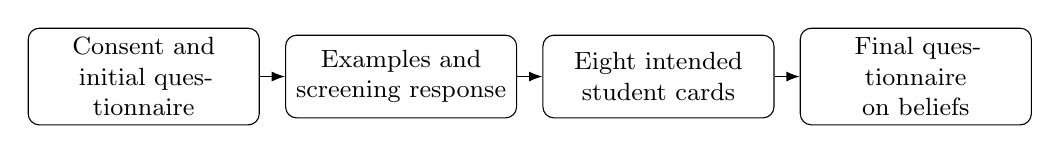
\begin{tikzpicture}[n/.style={draw,rounded corners,align=center,text width=2.7cm,minimum height=1.05cm,font=\small},>=Latex]
\node[n] (a) {Consent and\\initial questionnaire};
\node[n,right=0.32cm of a] (b) {Examples and\\screening response};
\node[n,right=0.32cm of b] (c) {Eight intended\\student cards};
\node[n,right=0.32cm of c] (d) {Final questionnaire\\on beliefs};
\draw[->] (a)--(b);\draw[->] (b)--(c);\draw[->] (c)--(d);
\end{tikzpicture}
\caption{\new{Timing of the measurements used in this paper. One survey encounter contains several modules; the diagram does not represent longitudinal waves. The shared study context is disclosed in Appendix~\ref{app:scope}.}}\label{fig:timelineA}
\end{figure}

\subsection{Recorded profile support and covariates}
The six binary characteristics are coded using the existing study vectors. The 64 possible identifiers represent 56 distinct attribute combinations under that coding. We retain this support rather than reconstruct unobserved profiles or treat every identifier as an independently randomized combination. Appendix~\ref{app:support} documents the implications. The within-teacher regression is consequently reported as an additive summary over the observed support. Its interpretation as a marginal causal attribute effect requires the relevant assignment and support assumptions; the existence of six binary variables alone does not establish those assumptions.

The baseline predictor set, $X_1$, contains educational stage, experience, tenure at the current school, gender, age, school ownership, a reported permanent public appointment indicator, and number of teaching groups. $X_2$ adds perceived teacher impact, self-reported empathy, and the effort-versus-luck item. The final specification adds the resource-skepticism composite. Larger values on the effort item indicate a stronger role attributed to effort. The resource composite averages standardized responses about excessive resources allocated to repeaters and ineffective additional resources, and is standardized again. Its two items correlate at 0.483 in the available observations; the composite summarizes related judgments rather than establishing a single validated latent construct.

We retain the existing harmonization of instrument versions: alternative impact items are combined, and empathy responses on the longer scale are mapped to the five-category scale. Age and experience enter jointly because the target is their conditional association. The public-employment item is described according to what was actually recorded; absence of a public appointment report is not evidence of a temporary private-sector contract.

\section{Decision framework and empirical strategy}
\begin{addition}
\subsection{Common information, differing judgments}
Let $x$ denote the information on a student profile and let $V_j(x)$ be teacher $j$'s perceived net educational value of recommending repetition rather than promotion. A simple representation is
\[
 Y_j(x)=\mathbf{1}\{V_j(x)+u_j(x)>0\}.
\]
Differences in $V_j(x)$ may arise from expected learning gains, perceived costs, beliefs about alternatives, or different interpretations of the same information. The term $u_j(x)$ accommodates response noise and omitted considerations. The framework is deliberately agnostic about whether disagreements are justified. It motivates three separate empirical objects: changes across presented attributes, disagreement at a given profile, and the predictability of a teacher's average response relative to comparable cases.

For a specified profile distribution $Q$, a population target could be written as
\[
 \theta_j(Q)=E_{x\sim Q}\{p_j(x)-\bar p(x)\},
\]
where $p_j(x)$ is a recommendation probability and $\bar p(x)$ is the comparison-population average. This target depends on both the reference population and $Q$. The available task estimates a finite-response analogue over each teacher's recorded cases. It does not identify $p_j(x)$ for all profiles or a context-free personal trait.
\end{addition}

\subsection{Attribute coefficients and same-profile disagreement}
At the card level, we estimate
\[
 Y_{ij}=\alpha_j+X_{ij}'\beta+\varepsilon_{ij},
\]
where $\alpha_j$ is a teacher fixed effect and $X_{ij}$ contains the six attributes. Each coefficient compares responses within teachers while adjusting for the other recorded attributes. Standard errors are clustered by teacher. The model uses 22,006 observations from 2,587 teachers; the 118 single-response teachers contribute no within-teacher variation. We retain the linear probability specification to report all coefficients in percentage points.

\new{Disagreement is measured separately from this regression. For a card with $n_i$ responses and $s_i$ recommendations to repeat, the probability that two distinct observed respondents disagree is $D_i=2s_i(n_i-s_i)/[n_i(n_i-1)]$. We average $D_i$ using observed card frequencies, and also report equal-identifier weighting. This is disagreement about an identical recorded card, not unexplained variance from a linear model. It is descriptive of the respondents and survey context.}

\subsection{Relative recommendation propensity}
\old{The preferred measure defines harshness as the average deviation from other teachers who evaluated the same card. We define it in two steps. First, for each teacher-card decision, we compute the distance between teacher \(j\)'s decision for card \(i\) and the leave-one-out repetition rate for that same card:}
\old{\[
d_{ij}=R_{ij}-\bar{R}_{i,-j}.
\]}
\old{Here, \(R_{ij}\) equals one if teacher \(j\) recommends repetition for card \(i\), and zero otherwise. The term \(\bar{R}_{i,-j}\) is the average repetition rate for card \(i\) among all other teachers who evaluated that same card, excluding teacher \(j\). Second, we average those distances across the cards evaluated by teacher \(j\):}
\old{\[
H^b_j=\frac{1}{n_j}\sum_{i\in I_j} d_{ij}.
\]}
We refer to $H^b_j$ as relative recommendation propensity. A value of 0.10 indicates an average recommendation ten percentage points above the leave-one-out rate for the recorded cards. The historical label ``harshness'' does not imply a normative judgment about whether repetition was appropriate.

\new{The index has useful limits and properties. It lies in $[-1,1]$; excludes the focal response from its comparison rate; and satisfies $\sum_j n_j H^b_j=0$ exactly when each recorded teacher-card response appears once. Its unweighted teacher mean need not be zero when response counts differ. Adjusting for card averages improves comparability but does not equalize measurement precision or remove sampling noise. We report teacher-level regressions with HC3 covariance and supplement their uncertainty with 399 teacher bootstrap draws that reconstruct the reference rates.}

We retain terciles of the observed index as a descriptive display. Ties produce groups of 908, 864, and 933 teachers. Because these groups are defined using the same decisions subsequently described, the resulting slopes do not independently validate latent types or estimate the effect of becoming more repetition-prone.

\begin{addition}
\subsection{Prediction for teachers outside the training sample}
All predictive models use the same 2,156 complete-case teachers. We create five teacher folds and repeat the partition three times. Within each training fold, the target uses leave-one-out profile rates calculated only from training teachers. For held-out teachers, the target subtracts the training profile rate from the teacher's responses. Thus a test teacher's responses cannot influence either the fitted model or its profile benchmark. Standardization of the resource composite is also fitted within training folds.

We compare a training-mean baseline, OLS, and random forests for $X_1$, $X_2$, and the full predictor set. Forests use 500 trees, a minimum terminal-node size of 20, and the square root of the predictor count, rounded down, as the candidate-variable count. These settings are fixed rather than selected using test outcomes. The performance measure is
\[
 R^2_{\mathrm{test}}=1-\frac{\sum_j(H_j^{\mathrm{test}}-\widehat H_j)^2}{\sum_j(H_j^{\mathrm{test}}-\overline H_{\mathrm{train}(j)})^2}.
\]
A negative value means the model performs worse than the training-mean prediction. The reported range across partitions measures sensitivity to fold assignment, not a confidence interval. SHAP values are calculated for held-out teachers using the full forest from the first partition, with training-only background observations. They are descriptive explanations of predictions, not an additional performance test.
\end{addition}

\section{Results}
\subsection{Academic information dominates the average recommendation}
Table~\ref{tab:attrA} reports the within-teacher coefficients. Three or more failed subjects have a coefficient of 54.62 points (95 percent interval 53.23 to 56.01); low basic competences have a coefficient of 27.07 (25.83 to 28.31). Frequent unjustified absence and serious disciplinary problems have smaller positive coefficients, 6.37 and 4.56 points respectively. A complex background is associated with a 1.88-point reduction conditional on the other attributes. The male-student coefficient is 0.26 points, with an interval from $-0.62$ to 1.15. This supports a small average gender contrast in the coded task, rather than the absence of every possible gender interaction.
\inputtab{revised}{A_attributes}{Within-teacher student-attribute coefficients}{tab:attrA}
The sizes distinguish the role of academic signals from behavioral and background information. They do not establish the optimal weights for actual educational decisions. Nor does the negative background coefficient identify empathy as a mechanism: different beliefs about causes, alternatives, or the costs of repetition can generate the same sign. The restricted no-scenario comparison in Appendix~\ref{app:scope} yields similar dominant academic coefficients.

\subsection{Comparable cases still generate disagreement}
The overall recorded repetition rate is 47.62 percent when decisions receive equal weight; the teacher-weighted average is 48.39 percent. The frequency-weighted probability of a disagreement between distinct teachers evaluating the same identifier is 25.89 percent, compared with 26.01 percent under equal-identifier weighting. Consequently, a clear aggregate hierarchy does not mean that individual recommendations coincide.

The relative-propensity distribution has a standard deviation of 20.97 points and an unweighted mean of $-0.61$ points. Figure~\ref{fig:distributionA} shows the distribution without imposing normality. There are 169 teachers whose retained responses never recommend repetition. That observed pattern is compatible with several explanations, including opposition to repetition, the cases observed, or limited response counts; it is not itself a measurement of a general belief.
\plot{revised}{propensity_distribution}{Distribution of relative recommendation propensity among 2,705 teachers. The distribution combines differing numbers of recorded responses.}{fig:distributionA}
Tercile summaries preserve an intuitive description of the sample (Appendix~\ref{app:terciles}). Teachers in the lower and upper groups recommend repetition on 25.87 and 70.13 percent of their recorded cases, respectively. Their average ages are 46.27 and 44.22 years. These summaries show differences in the realized responses and modest shifts in some characteristics; the large response contrast is partly built into how the groups are formed.

\subsection{Associations are detectable, but predictive gains are small}
Table~\ref{tab:charA} reports the full characterization model and the change in fit on the common sample. The $R^2$ rises from 2.73 percent for baseline characteristics to 3.06 percent with the additional belief measures and 4.22 percent with resource skepticism. On this same sample, adding variables improves in-sample fit only modestly.
\inputtab{revised}{A_characterization}{Teacher characteristics and relative recommendation propensity}{tab:charA}
Secondary-stage teaching is associated with 3.35 points higher relative propensity, age with $-0.30$ points per year holding experience and the other variables constant, effort attribution with 0.46 points per scale unit, and resource skepticism with 2.06 points per standard deviation. Bootstrap intervals that rebuild profile comparisons support the same broad associations. These are conditional associations, including with attitudes reported after the task. They do not establish effects of training, aging, or changing beliefs.

\begin{addition}
Table~\ref{tab:predA} presents the more demanding predictive comparison. The baseline root mean squared error is 18.54 points. OLS with all predictors reduces it to 18.26 points: a gain of approximately 0.28 points, or 1.5 percent of baseline RMSE. Its mean out-of-fold $R^2$ is 3.02 percent, ranging from 2.75 to 3.33 percent across partitions. The full forest achieves RMSE of 18.48 points and mean $R^2$ of 0.61 percent, with a range from $-0.07$ to 1.63 percent. Baseline-only and intermediate forests do not outperform the mean predictor on average.
\end{addition}
\inputtab{added}{A_prediction}{Prediction for held-out teachers on a common sample}{tab:predA}
\new{Allowing nonlinearities through this forest does not uncover a large hidden predictive signal. This comparison does not prove that every possible algorithm or unmeasured characteristic would fail. It establishes that the observed variables, under the documented linear and flexible specifications, offer limited improvement over a simple mean prediction. Resource skepticism, age, and educational stage have the largest mean absolute out-of-fold SHAP contributions in the full forest (Appendix~\ref{app:prediction}); that ranking should be read alongside the forest's small predictive gain.}

\subsection{Exploratory sequence analysis}
\new{Display-order metadata recover eight unique positions for 2,981 raw records, including 2,612 retained teachers. Adjacent observed responses produce 16,656 pairs. To assess alternation without mechanically attributing teacher demeaning to a behavioral mechanism, we examine 1,885 complete eight-response sequences. Decisions switch on 47.45 percent of adjacent pairs; 999 within-teacher permutations yield a mean of 47.14 percent and a two-sided permutation $p$ of 0.397. A negative lagged-decision coefficient from a short fixed-effect panel is not convincing evidence of compensatory behavior: reordering intact profile-response pairs produces similarly negative coefficients. Appendix~\ref{app:sequence} gives this benchmark. The evidence does not identify a general tendency to compensate for a preceding recommendation.}

\section{Discussion}
The findings separate three aspects of teacher judgment that are often combined. Academic difficulties strongly organize recommendations. Teachers nevertheless disagree on a meaningful share of identical recorded cases. Professional characteristics and reported beliefs predict only a small portion of the remaining between-teacher variation. The first finding concerns common response patterns, the second describes disagreement, and the third concerns the usefulness of observed information about teachers.

The standardized design strengthens this distinction relative to comparisons of teachers' raw administrative retention rates. The same recorded cases can be compared across teachers, and the fixed-effect analysis uses changes in student information within a teacher. This reduces the immediate confounding between decision propensity and the composition of a teacher's actual classroom. It does not measure all the information used in actual cases, test the correctness of recommendations, or establish their consequences.

The limited predictive signal also changes the interpretation of statistically detectable associations. An age coefficient or a resource-belief coefficient may be substantively interesting without allowing accurate classification of individual teachers. The results offer little basis for using this covariate set to identify teachers who will consistently recommend repetition more frequently. They do not imply that background characteristics are irrelevant in every setting, or that interventions targeting professional knowledge cannot matter.

\new{An important alternative explanation is measurement noise. A small number of responses per teacher produces an imperfect measure of a stable propensity, even if such a propensity exists. The target also changes with the set of cases and the comparison population. A low predictive $R^2$ for this finite-response measure therefore does not by itself distinguish weakly predictable stable differences from noisy measurement. Repeated independent tasks or longitudinal measurements would be necessary to estimate reliability and persistence convincingly.}

Several additional boundaries matter. The sample is voluntary and concentrated in a single region. Recorded examples remain in the outcome under the retained analysis rule. The current attribute coding does not constitute all 64 distinct combinations. Belief measures follow the decisions, and there is no reliable school identifier for clustering or separating shared institutional influences. Teacher-clustered uncertainty addresses repeated responses, but cannot rule out residual dependence between colleagues. These boundaries delimit the claims rather than eliminate the descriptive comparison the design makes possible.

\section{Conclusion}
Standardized profiles reveal strong common responses to academic difficulties alongside disagreement that observable teacher characteristics predict poorly. The evidence supports describing both the decision inputs and the limits of characterization. It does not support moving directly from significant covariate coefficients to a reliable typology of teachers. For research on repetition, the next step is to connect comparable-case judgments to repeated measurements and actual decisions, so that disagreement, persistence, and educational consequences can be studied separately.

\clearpage
\begingroup\color{revised}\begin{thebibliography}{99}\small
\bibitem{allen} C. S. Allen, Q. Chen, V. L. Willson, and J. N. Hughes, ``Quality of research design moderates effects of grade retention on achievement: A meta-analytic, multilevel analysis,'' \textit{Educational Evaluation and Policy Analysis}, vol. 31, no. 4, pp. 480--499, 2009. \href{https://doi.org/10.3102/0162373709352239}{doi:10.3102/0162373709352239}.
\bibitem{goos} M. Goos, J. Pipa, and F. Peixoto, ``Effectiveness of grade retention: A systematic review and meta-analysis,'' \textit{Educational Research Review}, vol. 34, art. 100401, 2021. \href{https://doi.org/10.1016/j.edurev.2021.100401}{doi:10.1016/j.edurev.2021.100401}.
\bibitem{tomchin} E. M. Tomchin and J. C. Impara, ``Unraveling teachers' beliefs about grade retention,'' \textit{American Educational Research Journal}, vol. 29, no. 1, pp. 199--223, 1992. \href{https://doi.org/10.3102/00028312029001199}{doi:10.3102/00028312029001199}.
\bibitem{bonvin} P. Bonvin, ``The role of teacher attitudes and judgement in decision-making: The case of grade retention,'' \textit{European Educational Research Journal}, vol. 2, no. 2, pp. 277--294, 2003. \href{https://doi.org/10.2304/eerj.2003.2.2.6}{doi:10.2304/eerj.2003.2.2.6}.
\bibitem{klapproth} F. Klapproth and C. Beyte, ``GPA, student gender, school subject, and teacher attitudes in grade retention decisions: An experimental study,'' \textit{European Journal of Psychology of Education}, vol. 41, art. 24, 2026. \href{https://doi.org/10.1007/s10212-026-01072-7}{doi:10.1007/s10212-026-01072-7}.
\bibitem{pajares} M. F. Pajares, ``Teachers' beliefs and educational research: Cleaning up a messy construct,'' \textit{Review of Educational Research}, vol. 62, no. 3, pp. 307--332, 1992. \href{https://doi.org/10.3102/00346543062003307}{doi:10.3102/00346543062003307}.
\bibitem{conjoint} J. Hainmueller, D. J. Hopkins, and T. Yamamoto, ``Causal inference in conjoint analysis: Understanding multidimensional choices via stated preference experiments,'' \textit{Political Analysis}, vol. 22, no. 1, pp. 1--30, 2014. \href{https://doi.org/10.1093/pan/mpt024}{doi:10.1093/pan/mpt024}.
\bibitem{validation} J. Hainmueller, D. Hangartner, and T. Yamamoto, ``Validating vignette and conjoint survey experiments against real-world behavior,'' \textit{Proceedings of the National Academy of Sciences}, vol. 112, no. 8, pp. 2395--2400, 2015. \href{https://doi.org/10.1073/pnas.1416587112}{doi:10.1073/pnas.1416587112}.
\bibitem{prediction} S. Mullainathan and J. Spiess, ``Machine learning: An applied econometric approach,'' \textit{Journal of Economic Perspectives}, vol. 31, no. 2, pp. 87--106, 2017. \href{https://doi.org/10.1257/jep.31.2.87}{doi:10.1257/jep.31.2.87}.
\bibitem{rf} L. Breiman, ``Random forests,'' \textit{Machine Learning}, vol. 45, pp. 5--32, 2001. \href{https://doi.org/10.1023/A:1010933404324}{doi:10.1023/A:1010933404324}.
\bibitem{shap} S. M. Lundberg and S.-I. Lee, ``A unified approach to interpreting model predictions,'' in \textit{Advances in Neural Information Processing Systems}, vol. 30, pp. 4765--4774, 2017. \url{https://papers.nips.cc/paper/7062-a-unified-approach-to-interpreting-model-predictions}.
\bibitem{nickell} S. Nickell, ``Biases in dynamic models with fixed effects,'' \textit{Econometrica}, vol. 49, no. 6, pp. 1417--1426, 1981. \href{https://doi.org/10.2307/1911408}{doi:10.2307/1911408}.
\end{thebibliography}
\endgroup
\clearpage\appendix
\section{Profile support and sample accounting}\label{app:support}
\begin{addition}
The retained coding maps 64 identifiers to 56 distinct attribute combinations. Two favorable-example identifiers are omitted from outcome construction. All remaining nonmissing binary decisions are retained, including partial responses and recorded unfavorable-example information. No synthetic observations are created for absent combinations. Profile benchmarks distinguish identifiers, following the existing analysis; pooling identical attribute combinations would define a different benchmark.

The complete file used for scores contains 22,124 decisions from 2,705 teachers. Counts by teacher are: one, 118; two, 16; three, 18; four, 6; five, 14; six, 10; seven, 154; eight, 633; nine, 1,736. Score construction does not require an observed policy ranking or complete final questionnaire. Baseline OLS can use 2,641 observations; the comparison of all predictor sets uses the common 2,156 cases. Missing covariates are not assigned artificial values in these characterization models. The score is calculated with the full retained reference population for the descriptive regressions, whereas predictive validation uses training-only reference populations.

For each card, writing $\bar R_i=s_i/n_i$ yields
\[
R_{ij}-\bar R_{i,-j}=\frac{n_i}{n_i-1}(R_{ij}-\bar R_i).
\]
Summing over the teachers observed for that card gives zero. Summing again across cards gives $\sum_j n_jH^b_j=0$. This is an algebraic centering property, not evidence of unbiased teacher-type measurement. Removing a focal teacher from its reference also does not make different teachers' scores statistically independent: they still share comparison observations. The teacher bootstrap reconstructs those comparisons in every draw.
\end{addition}

\section{Descriptive terciles and alternative outcomes}\label{app:terciles}
The terciles summarize realized responses. They use empirical one-third and two-thirds cutoffs while keeping ties together. The response-derived groups are not treated as exogenous moderators. Table~\ref{tab:tercA} reports their attribute coefficients without interpreting between-column differences as causal differences in teacher types.
\inputtab{revised}{A_terciles}{Student-attribute coefficients within observed score terciles}{tab:tercA}
Two alternative outcome summaries retain the same response sample: the unadjusted teacher average $H^a_j$ and the teacher average residual from a pooled logistic model of the six attributes, $H^c_j$. These quantities answer slightly different questions. The first retains profile-composition differences; the second uses a parametric rather than identifier-specific benchmark. Table~\ref{tab:altA} compares selected characterization coefficients, using the common complete-case covariates.
\inputtab{revised}{A_alternatives}{Selected associations across alternative outcome definitions}{tab:altA}

\section{Predictive specification and interpretation}\label{app:prediction}
\begin{addition}
The forest and OLS models use the original continuous age, experience, tenure, belief, and group-count variables rather than discretized terciles. Educational stage is categorical. All model comparisons use identical held-out teachers and identical fold-specific target construction. Each repetition contains one held-out prediction per teacher per model. The data therefore contribute 45,276 teacher-model-partition predictions, not 45,276 independent teachers.

The full forest's SHAP summary uses the first five-fold partition, 32 Monte Carlo simulations per feature, and 128 randomly sampled training-background observations per fold. The additive adjustment is applied within each explanation. No narrow confidence interval based on resampling a fixed fitted model is presented. Correlated predictors can share predictive contributions in multiple ways, so feature rankings do not identify unique causal mechanisms. Out-of-fold permutation-importance results are included in the replication tables as a complementary model diagnostic.
\end{addition}
\plot{added}{prediction}{Out-of-fold predictive performance. Bars show variation across three partitions, not sampling confidence intervals.}{fig:predictionA}
\plot{added}{shap}{Mean absolute SHAP contributions for held-out teachers in the full random forest. The model has limited overall predictive performance.}{fig:shapA}

\section{Recovered order and sequential dependence}\label{app:sequence}
\begin{addition}
Order fields identify the positions of cards within their assigned group. They recover presentation order, not a second answer to a question reused as an example. A valid sequence requires eight distinct identifiers and positions one through eight. Only adjacent positions with observed retained responses enter the pair analysis.

A regression of the current decision on the previous decision, teacher effects, current-card effects, and position indicators gives a lag coefficient of $-5.61$ points. Such a coefficient is vulnerable to short-panel demeaning effects; a lagged response is not an independently assigned treatment \cite{nickell}. On the common complete-eight sample, the model with teacher and current-card effects gives $-5.48$ points. Randomly reassigning positions to intact profile-response pairs within teachers 199 times yields a mean coefficient of $-6.44$ points and a central 95 percent permutation range from $-7.60$ to $-5.24$ points. The two-sided permutation comparison gives $p=0.12$.

This descriptive reference preserves each teacher's decisions and the profile-response mapping while removing their observed sequence. Its negative mean demonstrates why the raw negative slope should not be interpreted as moral licensing or aversion to consecutive repetition recommendations. The permutation analysis is exploratory and is not a design-based randomization test of a psychological mechanism under every possible survey-order constraint.
\end{addition}

\section{Shared-study disclosure and restricted-sample check}\label{app:scope}
\begin{addition}
The data also support the companion manuscript \textit{Policy Scenarios, Preference Elicitation, and Grade-Repetition Recommendations}. That paper analyzes between-teacher scenario assignments and the timing of policy rankings. The present paper develops neither those treatment results nor their narrative. For transparency, its main descriptive analysis pools the study contexts. A sensitivity analysis restricted to the no-policy-assignment control uses 281 teachers with a score and 2,292 identifying within-teacher observations from 274 teachers. The two dominant attribute coefficients are 54.07 points for failed subjects and 26.76 points for low competences; their 95 percent intervals are [49.63, 58.51] and [22.96, 30.56]. This supports the central academic-information pattern without requiring a claim that all survey contexts have identical effects.

The initial analysis plan and questionnaire are available in the project materials. The current decomposition into two papers, common-sample predictive validation, reconstructed-reference bootstrap, and sequence diagnostics are subsequent analyses. We do not characterize them as prospectively registered tests. Replication scripts, aggregate tables, and this manuscript are maintained separately from the original analysis files. No public release of teacher-level records is presumed by the working draft.
\end{addition}
\end{document}
